\section{Evaluation}

\subsection{Microbenchmarks}
\label{q_microbenchmarks}

We evaluate all the queue implementations on a set of microbenchmarks to determine their scalability and performance. The controlled nature of these microbenchmarks allows us to compare particular aspects of each algorithm, such as transactional overhead introduced by STO. All experiments are run on a 100GB DRAM machine with two 6-core Intel Xeon X5690 processors clocked at 3.47GHz. Hyperthreading is enabled in each processor, resulting in 24 available logical cores. The machine runs a 64-bit Linux 3.2.0 operating system, and all benchmarks and STO data structures are compiled with \texttt{g++-5.3}. In all tests, threads are pinned to cores, with at most one thread per logical core.
In all graphs, we show the median of 5 consecutive runs with the minimum and maximum performance results represented as error bars.

\subsubsection{Parameters}

\emph{Value Types}. Each queue benchmark uses randomly chosen integers because the benchmarks do not manipulate the push or popped values and the queue algorithms are agnostic to the actual values being placed in the queue.

\emph{Initial Queue Size}. We run our tests with varying numbers of initial entries in the queue. This affects how often the structure becomes empty, which can cause aborts and additional overhead (as described in the algorithms above). It also affects the number of cache lines accessed: a near-empty queue will never require iterating over values contained in more than one cache line.

\emph{Operations per transaction}. We set the number of operations per transaction to 1 (i.e., the transactions are singleton transactions). By keeping a transaction as short as possible, we maximize the impact of any fixed per-transaction overhead. However, we also minimize the performance hit from the additional transactional overhead required to maintain and commit larger read- or write-sets: running multiple-operation transactions requires multiple-item support in read- and write-sets, creates scenarios of read-my-writes, and increases the number of aborts and retries, all of which incur additional overhead. 
Because most highly-concurrent data structures provide guarantees equivalent to those of singleton transactions, we use singleton transactions when comparing transactional and non-transactional data structures.
Note that our data structure implementations can correctly handle multiple-operation transactions: we simply benchmark them with singleton transactions to compare performance.

\subsubsection{Tests}
    \emph{2-Thread Push-Pop Test}. This test has one thread that performs only pushes and another thread that performs only pops (a traditional ``producer-consumer'' model). Each thread performs 10 million transactions. Unless the queue is empty, the two threads should never be modifying the same part of the data structure and will never conflict, leading to an abort rate that should be near 0. We use this test to measure the speed of push/pops on the queue under low or no contention. We expect that our transactional queues should perform just as well as the highly-concurrent queues, if not better: while highly-concurrent, non-transactional algorithms are optimized for multi-threaded access, our simpler implementation should be just as fast with low contention and low abort rates.

\emph{Multi-Thread Singletons Test}.
    In this test, a thread randomly selects an operation (push or pop) to perform within each transaction. This keeps the queue at approximately the same size as its initial size during the test. Each thread performs 10 million transactions. We run this test with different initial queue sizes and different numbers of threads, with each thread performing singleton transactions. Altering the number of threads allows us to benchmark performance under variable amounts of contention. We expect that T-QueueO and T-QueueP queues will perform significantly worse once the number of threads is increased, and that these naive synchronization algorithms will underperform synchronization algorithms optimized for contentious situations.

\subsection{Overview of Results}

We first present an overview of our conclusions, then explaining each conclusion in more detail by proposing a sequence of five hypotheses tested using the benchmarks described above. For each hypothesis, we use our benchmark results to formulate a conclusion that either refutes or supports the hypothesis.
We provide a few figures that highlight our results; full results (including abort rates) can be found in Appendix~\ref{app:queues}. We draw the following conclusions from our results:
\begin{itemize}
    \item Performance improves when implementing contentious operations with a pessimistic, rather than optimistic, approach.
    \item Fixed overhead from bookkeeping STO wrapper calls is negligible.
    \item The flat combining technique is a highly effective synchronization technique for queues, and the flat combining, non-transactional queue outperforms all transactional and concurrent queues.
    \item Performance of the transactional flat combining queue underperforms all transactional queues. The performance loss comes from the greater number and greater complexity of flat combining calls that are necessary to convert the non-transactional flat combining queue to a transactional one.
\end{itemize}

\subsection[Hypothesis 1]{Hypothesis 1}
\subsubsection{A transactional queue using a pessimistic algorithm for pop achieves better performance than one using an optimistic algorithm for pop (Supported).}

We test this hypothesis by comparing the performance of T-QueueO and T-QueueP queue. These two queues differ only in that a thread running on T-QueueP queue locks the queue immediately when it performs a transactional pop, therefore pessimistically assuming that any other thread accessing the queue will cause a conflict with its pop operation.

\begin{figure}[t!]
    \centering
	\begin{minipage}{\textwidth}
        {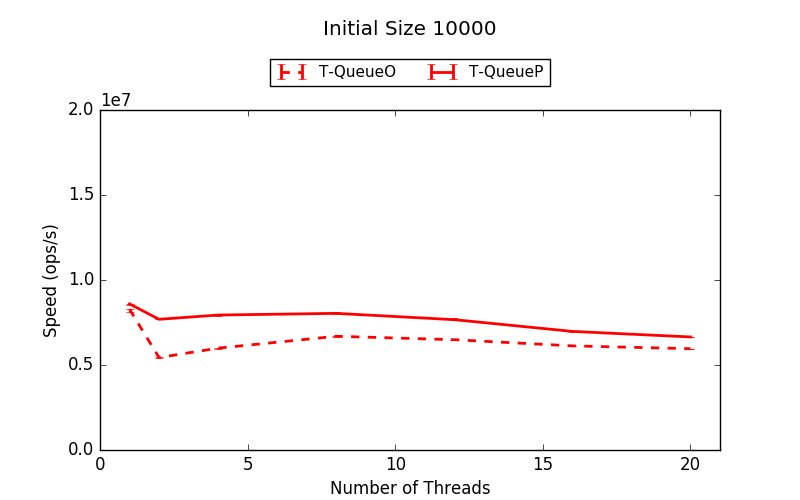
\includegraphics[width=\textwidth]{fcqueues/stoQ:RandSingleOps10000.png}}
	\end{minipage}
    \caption{T-QueueO vs. T-QueueP Performance: Multi-Thread Singletons Test}
    \label{fig:stoqs}
\end{figure}

The comparative performance of T-QueueO and T-QueueP (Figure~\ref{fig:stoqs}) on the Multi-Thread Singletons Test demonstrates that using a pessimistic technique for transactional pop execution is more effective than an optimistic one. T-QueueP performs slightly better than T-QueueO on the Multi-Thread Singletons Test. This is likely due to T-QueueP's lower abort rate (1/3 that of T-QueueO): a pop in T-QueueP locks the queue and prevents any other thread from observing an inconsistent state. The T-QueueO allows threads to observe inconsistent state (i.e., execute a pop of a head that is about to be popped by another thread); this causes aborts at execution and commit time.
This result supports that a pessimistic approach to contentious operations such as pop benefits performance.

\begin{figure}[t]
    \centering
	\begin{minipage}{\textwidth}
        {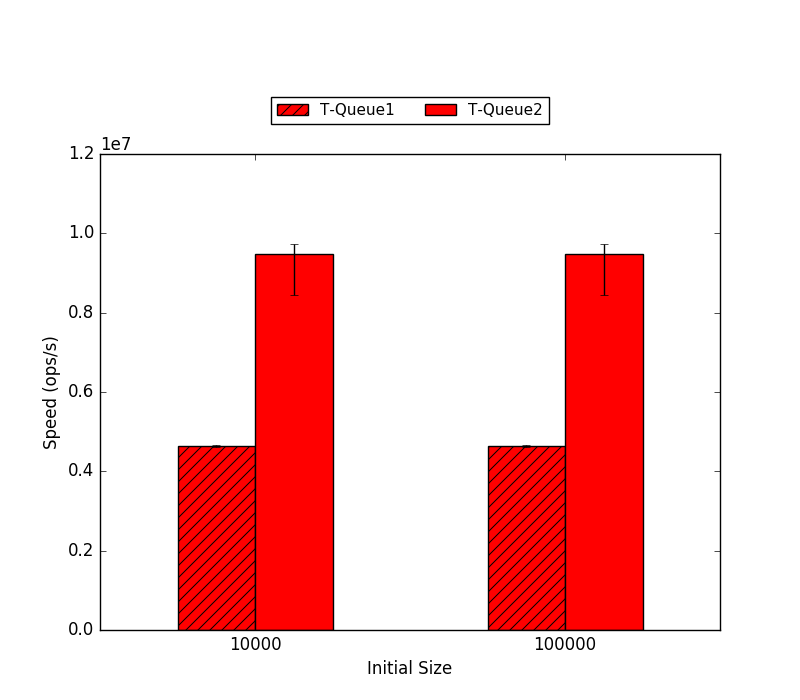
\includegraphics[width=\textwidth]{fcqueues/stoQ:PushPop.png}}
	\end{minipage}
    \caption{T-QueueO vs. T-QueueP Performance: Push-Pop Test (2 threads)}
    \label{fig:stoqs_pp}
\end{figure}

    On the Push-Pop Test, T-QueueP's performance is double that of T-QueueO's performance (Figure~\ref{fig:stoqs_pp}). This result is initially surprising, because the Push-Pop Test is a low-contention test (the abort rates, as expected, are near 0, with aborts only occurring because the threads spin too long while acquiring locks). We should therefore expect that T-QueueP performs approximately equal to T-QueueO. However, this is clearly not the case.

\begin{figure}[t]
    \centering
        {\includegraphics[width=\textwidth]{progress.png}}
    \caption{T-QueueO vs.\ T-QueueP Push-Pop Test: Speed at which the push- and pop-only threads complete 10 million transactions}
    \label{fig:sto_progress}
\end{figure}

Our results for the Push-Pop Test can be explained by the different speeds of the push and pop operations in T-QueueO and T-QueueP. Figure~\ref{fig:sto_progress} shows that T-QueueP's push-only thread performs approximately 10 million pushes per second, while T-QueueO's push-only thread performs only approximately 3.1 million pushes per second. T-QueueP's pop-only thread, \emph{when simultaneously running with the push-only thread}, performs only approximately 0.2 million pushes per second, while T-QueueO's pop-only thread, when running simultaneously with the push-only thread, performs approximately 2 million pushes per second.
Once the push-only thread exits, however, both queues' pop-only threads perform pops at a speed of about 10 million pops per second.

This data shows that T-QueueP's pop-only thread performs only 28 pops for every 100 pushes the push-only thread performs when the threads are running simultaneously, while T-QueueO's pop-only thread performs 64 pops for every 100 pushes the push-only thread performs when the threads are running simultaneously (Table~\ref{tab:sto_pop_push_ratio}). In addition, T-QueueP's pushes execute much faster than T-QueueO's, and pops in both queues---when the push-only thread has exited---execute at the same rate.

\begin{table}[t]
        \centering
    \begin{tabular}{|cc|}
        \hline
        Queue & Pops:Pushes\\
        \hline
            T-QueueO & 64:100\\
            T-QueueP & 28:100\\
        \hline
    \end{tabular}
    \caption{T-QueueO vs.\ T-QueueP Push-Pop Test: Ratio of pops to pushes when the push-only and pop-only threads are executing simultaneously}
    \label{tab:sto_pop_push_ratio}
\end{table}

The increased speed of a pop once the push-only thread has exited can be explained by the decrease in contention when only one thread is executing. The speed of a pop when the push-only thread is no longer executing is equal to the speed of a single-threaded pop execution. Single-thread execution on the queue results in better cache line performance (there can never be cache line bounces, because only one thread accesses the queue); furthermore, there is zero contention on the queue locks. 

T-QueueP's pushes execute significantly faster than do T-QueueO's, and the pushes also appear to be preventing T-QueueP's pops from executing quickly. This is because T-QueueP uses only one queue version as a global queue lock. Both a push and pop contend on this lock in order to install an operation; the push-only thread can potentially starve the pop-only thread by continuously succeeding in acquiring the lock.
Because of this starvation property, the push-only thread and pop-only thread in T-QueueP run in nearly a sequential fashion, with the push-only thread running first, and the pop-only thread running second.
Sequential execution, as discussed earlier, achieves better performance because of the lack of contention.
T-QueueP therefore has greater performance because its threads run in nearly a sequential fashion.\footnote{We note that T-QueueP's execution pattern also has the fortunate side effect of decreasing the probability that the queue becomes empty, since a greater number of pushes complete for every pop operation that completes.}

T-QueueO, on the other hand, uses two versions (head and tail versions) as locks, and each thread acquires only one of these locks when performing an operation. This allows both threads to execute operations at a more equal rate, since one cannot starve the other. However, because of the added contention on the cache lines containing the head and tail of the queue, both the push-only and pop-only threads execute at rates far slower than sequential execution.

We conclude that the unexpected results of the Push-Pop test are caused by the shared lock used by T-QueueP's push and pop operations that allow for a near-sequential execution of 10 million pops followed by 10 million pushes. This comes from our choice of implementation for the pessimistic pop algorithm, rather than the inherent pessimistic nature of the pop. Nevertheless, our results from the Multi-Thread Singletons Test do support our hypothesis. They indicate that a pessimistic approach does reduce the abort rate and lead to slightly better performance when two threads are both attempting to perform pops.

\vspace{12pt}
\noindent\fbox{\begin{minipage}{\textwidth}
    \textbf{SUPPORTED}: T-QueueP outperforms T-QueueO, indicating that a pessimistic approach is more appropriate for contentious operations such as pop.
\end{minipage}}


\subsection{Hypothesis 2}
\subsubsection{Hypothesis 2: Under low contention, a transactional queue with a naive concurrent algorithm performs reasonably well compared to the best concurrent, non-transactional queue algorithms (Supported).}

We benchmark a set of the best-performing highly-concurrent queue algorithms against our transactional queue implementations, T-QueueO and T-QueueP, using our low-contention test (the 2-Thread Push-Pop test) that is also optimized for a low abort rate. This acts as a best-case scenario for T-QueueO and T-QueueP algorithms. Selected results are shown in Figure~\ref{fig:ntqs_pp}.

Our implementation of the non-transactional flat combining queue, which we call NT-FCQueue, uses the flat combining queue implemented by the authors of the flat combining paper~\cite{flatcombining} (with minor modifications to remove memory leaks). Our implementations of the other highly-concurrent queues are taken from the open source Concurrent Data Structures (CDS) library implementations~\cite{libcds}. 

\begin{figure}[t!]
    \centering
	\begin{minipage}{\textwidth}
        {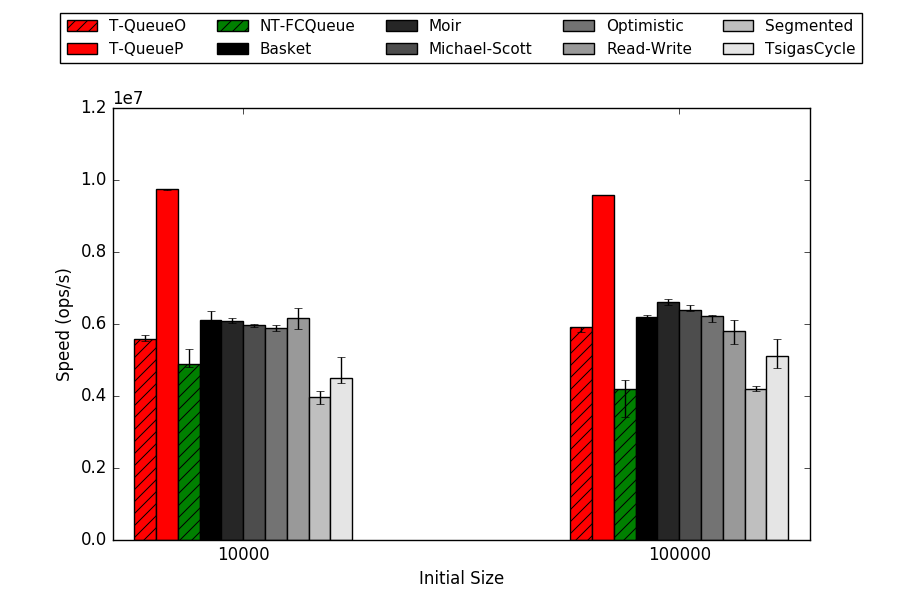
\includegraphics[width=\textwidth]{concurrent/allQ:PushPop.png}}
	\end{minipage}
    \caption{Non-transactional, Concurrent Queue vs.\ Transactional Queue Performance: Push-Pop Test (2 threads)}
    \label{fig:ntqs_pp}
\end{figure}

All concurrent, non-transactional queues achieve approximately equal performance on the Push-Pop Test besides NT-FCQueue, Segmented Queue~\cite{queue4}, and TsigasCycle Queue~\cite{queue5}. 
The T-QueueP outperforms all queues by at least 150\% on the 2-thread Push-Pop test. This is, as we discussed earlier, likely caused by T-QueueP's near-sequential execution on this test. We see in Table~\ref{tab:push_pop_ratio} that most queues perform more than 1 pop for every 2 pushes while the push-only thread is running. We also observe that NT-FCQueue is the only queue in which 10 million pops complete faster than 10 million pushes, and has nearly a 1:1 ratio of pops to pushes. This may explain its poor performance on the Push-Pop test as compared to the other queues (fewer pop operations are executed in a single-threaded manner after the push-only thread has exited).

\begin{table}[t]
        \centering
    \begin{tabular}{|cc|}
        \hline
        Queue & Pops:Pushes\\
        \hline
            T-QueueO & 64\\
            T-QueueP & 28\\
            NT-FCQueue & 110:100\\
            Basket & 42:100\\
            Moir & 62:100\\
            Michael-Scott& 54:100\\
            Optimistic & 50:100\\
            Read-Write & 84:100\\
            Segmented & 50:100\\
            TsigasCycle & 52:100\\
        \hline
    \end{tabular}
    \caption{Non-transactional Queues vs.\ T-QueueO and T-QueueP Push-Pop Test: Ratio of pops to pushes when the push-only and pop-only threads are executing simultaneously}
    \label{tab:push_pop_ratio}
\end{table}

Regardless of the difference in speed between the push-only and pop-only threads, we see that our naive algorithms perform at least as well as the majority of concurrent algorithms on this test. 
T-QueueO performs about equally as well as any non-transactional queue, and the ratio of pops to pushes in T-QueueO is close to that of these non-transactional queues.

The Push-Pop Test is designed for low abort rates and minimal transactional overhead from tracking items in read- and write-sets. It is therefore unsurprising that, on this test, a simple synchronization strategy can outperform the majority of highly-concurrent algorithms which are optimized for scalability. 
Our results demonstrate that a simple implementation of a naive algorithm can consistently outperform more complex concurrent queue implementations, even when supporting transactions using STO. The overhead added from STO does not inherently cripple performance---our transactional data structures can compete with several highly-concurrent, non-transactional data structures in particular cases. 

\vspace{12pt}
\noindent\fbox{\begin{minipage}{\textwidth}
    \textbf{SUPPORTED}: T-QueueP and T-QueueO outperform or match the performance of all concurrent, non-transactional queues on the 2-Thread Push-Pop Test. This indicates that a simple concurrent algorithm in a transactional setting can perform well under optimal circumstances.
\end{minipage}}


\newpage
\subsection{Hypothesis 3}
\subsubsection{The flat combining algorithm is the most promising concurrent queue algorithm to integrate with STO (Supported).}
\label{eval:hypo3}

\begin{figure}[t!]
    \centering
   	\begin{minipage}{\textwidth}
        {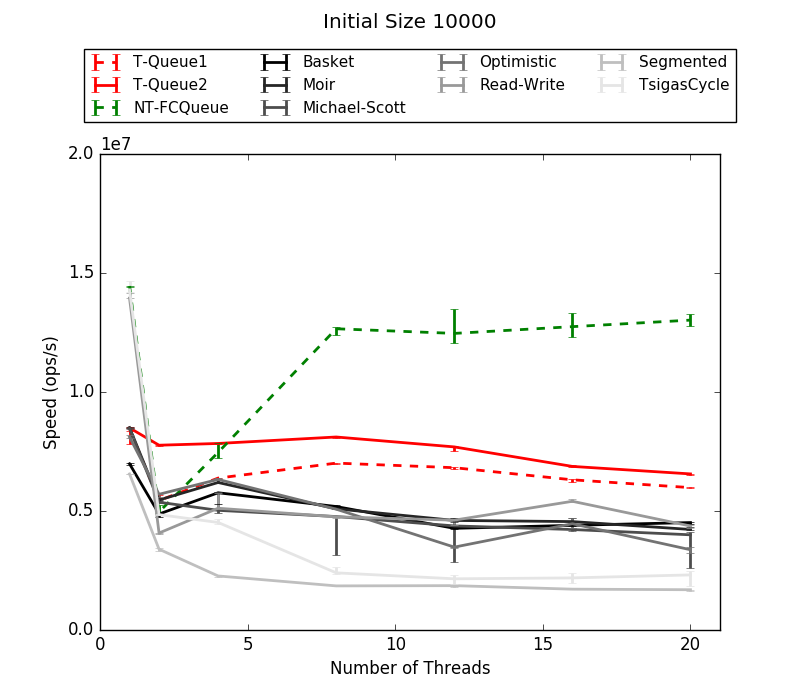
\includegraphics[width=\textwidth]{concurrent/allQ:RandSingleOps10000.png}}
	\end{minipage}
    \caption{Non-transactional, Concurrent Queue vs.\ Transactional Queue Performance: Multi-Thread Singletons Test}
    \label{fig:ntqs}
\end{figure}

We run the same set of highly-concurrent queues from the previous hypothesis on the Multi-Thread Singletons Test, which provides a more realistic example of high-contention workloads that a queue may experience. We investigate how different concurrent, non-transactional algorithms perform in high-contention situations compared to the transactional T-QueueP, and look for the most scalable and performant high-concurrency queue that outperforms T-QueueP to integrate with STO. Selected results are shown in Figure~\ref{fig:ntqs}.

On this test, NT-FCQueue achieves performance over 2.5$\times$ greater than any other concurrent, non-transactional queue as the number of threads increases above 2. The Multi-Thread Singletons Test highlights the performance benefits of the flat combining queue: as contention increases, the flat combining queue reaches performance approximately double that of T-QueueP. In addition, the flat combining queue is the only queue that scales. All the other highly-concurrent algorithms perform worse than T-QueueP, regardless of the number of threads accessing the queue or the initial queue size. 
Although an increase in the duration of a transaction and number of operations per transaction causes T-QueueP to perform far worse than other concurrent queues, our results demonstrate that a simple synchronization algorithm can achieve equal performance to more complex synchronization algorithms on our benchmarks.\footnote{We rely on the specific libcds~\cite{libcds} implementation of these concurrent, non-transactional data structures, which may not be the most optimized versions of these data structures. However, the performance of these implementations on our tests matches their performance in other research evaluating these data structures~\cite{queue1, queue3}.}

A comparison with NT-FCQueue indicates that the concurrent queue algorithms in T-QueueO and T-QueueP are certainly not optimal for performance in a non-transactional setting.
Given these results, as well as the algorithmic benefits of the flat combining technique described in Section~\ref{fcqueuent}, we choose the flat combining queue to integrate with STO.

\vspace{12pt}
\noindent\fbox{\begin{minipage}{\textwidth}
    \textbf{SUPPORTED}: NT-FCQueue significantly outperforms all highly-concurrent, non-transactional queues \emph{and} T-QueueP on the Multi-Thread Singletons Test, indicating that flat combining may be the most promising algorithm to integrate with STO to create a more performant and scalable transactional queue. 
\end{minipage}}

\subsection{Hypothesis 4}
\subsubsection{Overhead from general STO bookkeeping does not cripple performance of a highly-concurrent queue algorithm (Supported).}

We create a version of NT-FCQueue, called NT-FCQueueWrapped, that invokes general STO bookkeeping calls. The relative performance of NT-FCQueueWrapped to NT-FCQueue indicates how much of the overhead added by the STO system is unavoidable (without modifying STO itself). 

\begin{figure}[t!]
\centering
\singlespace
\lstset{
	language=C++,
	basicstyle=\ttfamily\small,
	keywordstyle=\color{blue}\ttfamily,
	stringstyle=\color{red}\ttfamily,
	commentstyle=\color{green}\ttfamily,
	morekeywords={true, false},
}
	\begin{lstlisting}
                    Sto::start_transaction();
                    try {
                        do_queue_op(push, 1);
                        do_queue_op(pop, 0);
                        if (Sto::try_commit()) {
                            printf("committed");
                        }
                    } catch (Transaction::Abort e) {
                        printf("aborted");
                    }
	\end{lstlisting}
\caption{Example usage of STO wrapper calls}
\label{fig:wrappers}
\end{figure}
The STO wrapper functions called by NT-FCQueueWrapped must be called by any user of the data structure in order for the data structure to perform the necessary bookkeeping to support transactions.
These two calls are \texttt{start\_transaction} and \texttt{try\_commit}, and allow a user to mark which operations should occur together in the same transaction. An example of how these calls are used are in Figure~\ref{fig:wrappers}. After invoking the \texttt{start\_transaction} call, the thread is able to collect items in its read- and write-sets. At the end of a transaction, the thread invokes the \texttt{try\_commit} call to run the commit protocol. The NT-FCQueueWrapped adds no items to the read- and write-sets after invoking \texttt{start\_transaction} and does nothing in its commit protocol. This means that NT-FCQueueWrapped incurs the minimum amount of overhead necessary to use STO and therefore represents the upper bound on the performance we can expect from a fully transactional flat combining queue (T-FCQueue). 

\begin{figure}[t!]
    \centering
   	\begin{minipage}{\textwidth}
        {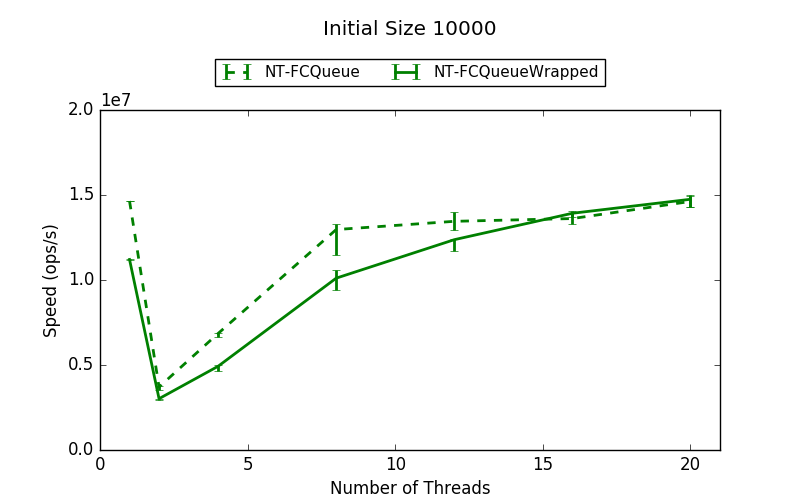
\includegraphics[width=\textwidth]{fcqueues/ntQ:RandSingleOps10000.png}}
	\end{minipage}
   \caption{NT-FCQueue vs. NT-FCQueueWrapped Performance: Multi-Thread Singletons Test}
    \label{fig:wrappedqs}
\end{figure}


We see from our Multi-Thread Singletons Test results (Figure~\ref{fig:wrappedqs}) that the STO wrapper calls can lead to a loss of performance ranging from 0\% at twenty threads to 30\% at four threads compared to the performance of the vanilla non-transactional flat combining queue. 
 With fewer threads accessing the queue, the proportion of overhead from the STO wrapper calls is greater because the overhead from synchronizing access to the queue is minimal. As the number of threads increases, the STO wrapper call overhead becomes negligible in comparison to the cost of synchronization.
NT-FCQueueWrapped retains most of NT-FCQueue's scalability, and the two queues perform equally well after the number of threads reaches approximately 14.

We also see an impact on performance of NT-FCQueue in the Push-Pop Test, shown in Figure~\ref{fig:wrappedqs_pp}: performance drops by approximately 20\%. The push-only thread now beats the pop-only thread in NT-FCQueueWrapped, but the ratio is still close to one pop operation performed per push operation (Table~\ref{tab:nt_pop_push_ratio}). The performance impact likely comes form the overhead added by STO wrapper calls; this is expected, as we discussed before, because this constant overhead more significantly affects performance at low thread counts and low contention.


\begin{figure}[t!]
    \centering
	\begin{minipage}{\textwidth}
        {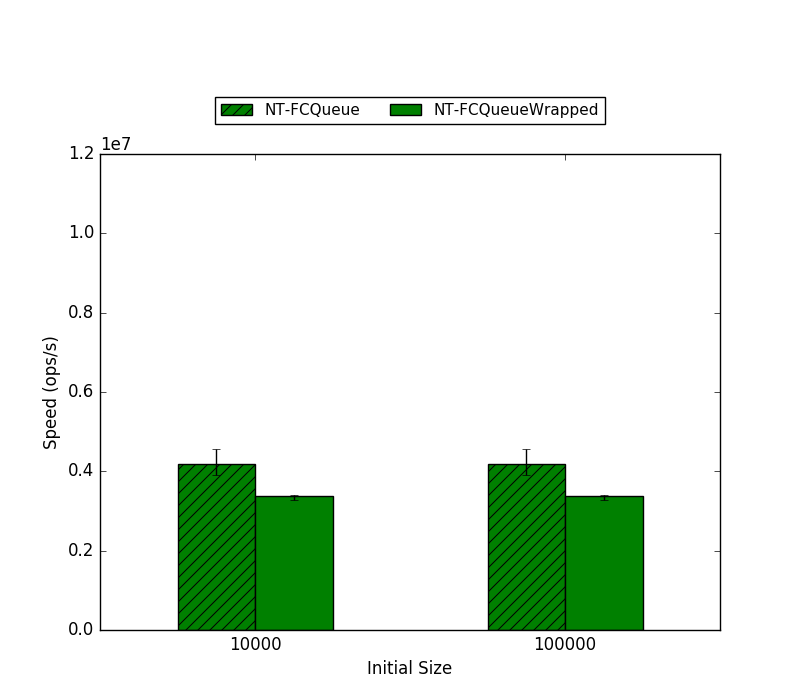
\includegraphics[width=\textwidth]{fcqueues/ntQ:PushPop.png}}
	\end{minipage}
    \caption{NT-FCQueue vs. NT-FCQueueWrapped Performance: Push-Pop Test (2 threads)}
    \label{fig:wrappedqs_pp}
\end{figure}
\begin{table}[ht!]
        \centering
    \begin{tabular}{|cc|}
        \hline
        Queue & Pops:Pushes\\
        \hline
            NT-FCQueue & 110:100\\
            NT-FCQueueWrapped & 94:100\\
        \hline
    \end{tabular}
    \caption{NT-FCQueue vs.\ NT-FCQueueWrapped Push-Pop Test: Ratio of pops to pushes when the push-only and pop-only threads are executing simultaneously}
    \label{tab:nt_pop_push_ratio}
\end{table}


Comparing NT-FCQueueWrapped and NT-FCQueue demonstrates that STO introduces unavoidable overhead that becomes negligible at high thread counts. Even with the wrapper calls, our results indicate it can still be possible to achieve performance up to nearly 2$\times$ greater at 20 threads than that of T-QueueP (the second-best performing queue).

\vspace{12pt}
\noindent\fbox{\begin{minipage}{\textwidth}
    \textbf{SUPPORTED}: Adding the calls to the general STO wrapper functions that are necessary for any data structure to support transactions does not cripple the performance of highly-concurrent queues such as NT-FCQueue, particularly at high thread counts.
\end{minipage}}

\subsection{Hypothesis 5}
\subsubsection{A transactional flat combining queue outperforms and scales better than a transactional queue with a naive concurrent algorithm (Not Supported).}
\label{eval:hypo5}

We compare T-FCQueue against NT-FCQueueWrapped and T-QueueP to measure how the flat combining transactional approach described in Section~\ref{fcqueuet} performs.

In the Push-Pop Test (Figure~\ref{fig:tqs_pp}), T-QueueP outperforms both flat combining variants. This is an unsurprising result given our results from the concurrent queues benchmark in Figure~\ref{fig:ntqs_pp}, and the fact that T-FCQueue has a more equal ratio of pops to pushes than does T-QueueP (Table~\ref{tab:tfc_pop_push_ratio}). 

\begin{figure}[t!]
    \centering
	\begin{minipage}{\textwidth}
        {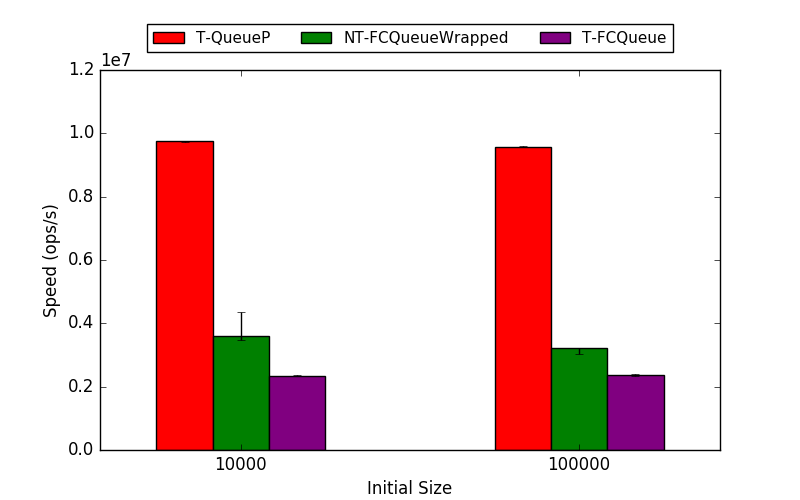
\includegraphics[width=\textwidth]{fcqueues/tQ:PushPop.png}}
	\end{minipage}
        \caption{T-FCQueue Performance: Push-Pop Test}
        \label{fig:tqs_pp}
\end{figure}

The Multi-Threaded Singletons Test (Figure~\ref{fig:tqs}) shows that T-QueueP performs approximately 2$\times$ better than T-FCQueue, regardless of initial queue size. Both queues do not scale, and the performance ratio remains constant regardless of the number of threads. The T-FCQueue also experiences abort rates around 5\%, which are $1.5$--$2\times$ the abort rates of T-QueueP.

\vspace{12pt}
\noindent\fbox{\begin{minipage}{\textwidth}
\textbf{NOT SUPPORTED}: The transactional flat combining queue does not outperform or scale better than other transactional queues using naive synchronization mechanisms. The T-FCQueue's poor performance compared to that of T-QueueP demonstrates that the flat combining algorithm performs poorly when modified to support transactions.
\end{minipage}}

\begin{table}[t!]
        \centering
    \begin{tabular}{|cc|}
        \hline
        Queue & Pops:Pushes\\
        \hline
            T-QueueP & 28:100\\
            NT-FCQueueWrapped & 94:100\\
            T-FCQueue & 57:100\\
        \hline
    \end{tabular}

    \caption{T-FCQueue Push-Pop Test: Ratio of pops to pushes when the push-only and pop-only threads are executing simultaneously}
    \label{tab:tfc_pop_push_ratio}
\end{table}


\begin{figure}[t!]
    \centering
   	\begin{minipage}{\textwidth}
        {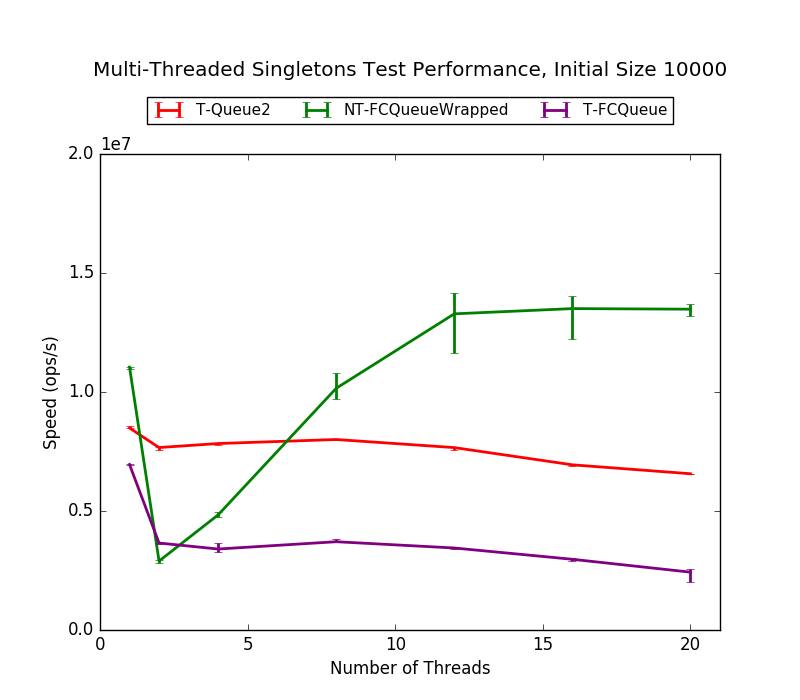
\includegraphics[width=\textwidth]{fcqueues/tQ:RandSingleOps10000.png}}
	\end{minipage}
    \caption{T-FCQueue Performance: Multi-Thread Singletons Test}
    \label{fig:tqs}
\end{figure}

\subsection{Conclusion}
Analysis with the \texttt{perf} tool indicates that the majority of T-FCQueue's overhead comes from spinning on the flat combining lock (acquired by the combiner thread) or waiting for a flat combining call to complete. In addition, the number of cache misses is over 4$\times$ greater than that of NT-FCQueue (see Figure~\ref{fig:qcm}). This overhead occurs for two reasons:
\begin{enumerate}
    \item \emph{Higher Quantity}: As described in Section~\ref{fcqueuet}, a thread must make multiple flat combining calls to perform a pop within a transaction (recall that a push only requires one flat combining call).
\item \emph{Higher Complexity}: each flat combining call requires executing instructions, which makes each operation request more expensive.
\end{enumerate}

We conclude that the flat combining technique, while perhaps near-optimal for a highly-concurrent data structure, is no better in a transactional setting than a naive synchronization technique such as that used in T-QueueO and T-QueueP. The flat combining algorithm must track the state of the queue during the transaction's lifetime to provide transactional guarantees (e.g., marking values in the queue or observing that the queue was empty when performing a pop). To do so requires both adding new flat combining calls and increasing the complexity of existing ones; these modifications cripple flat combining's performance.
In the next chapter, we formalize this argument using commutativity and claim that the flat combining technique fundamentally depends on operation commutativity present in only a non-transactional setting to achieve its high performance. 
